\section{Experimental Results}
\label{sec:ocnn_experiment-results}

In this section, we present empirical results produced by OC-NN model on synthetic and real data sets. We perform a comprehensive set of experiments to demonstrate that on complex data sets OC-NN performs on par with state-of-the-art methods and outperformed conventional shallow methods in some scenarios.
%%%%% Synthetic Dataset
\subsection{\tt OC-NN for Synthetic Data}
Single cluster consisting of 190 data points using $\mu=0$ and $\sigma = 2$ are generated as normal points , along with 10 anomalous points drawn from normal distribution with $\mu=0$ and $\sigma = 10$ having  dimension $d=512$. Intuitively, the latter normally distributed points are treated as being anomalous, as the corresponding points have different distribution characteristics to the majority of the training data. Each data point is flattened as a row vector, yielding a 190 $\times$ 512 training matrix and 10 $\times$ 512 testing matrix. We use a simple feed-forward neural network model with one-class neural network  objective as per Equation~\ref{eqn:oc-nn}.\\
%using network parameter settings described in Section~\ref{sec:feed forward oc-nn-model-config}.\\
\textbf{Results}.
From Figure~\ref{fig:synthetic-histogram}, we see that it is a near certainty for all $10$ anomalous points, are accurately identified as outliers with decision scores being negative for anomalies. It is evident that, the OC-NN formulation performs on par with classical OC-SVM in detecting the anomalous data points. In the next sections we apply to image and sequential data and demonstrate its effectiveness.


%% Results for Synthetic dataset
\begin{figure}
    \centering
    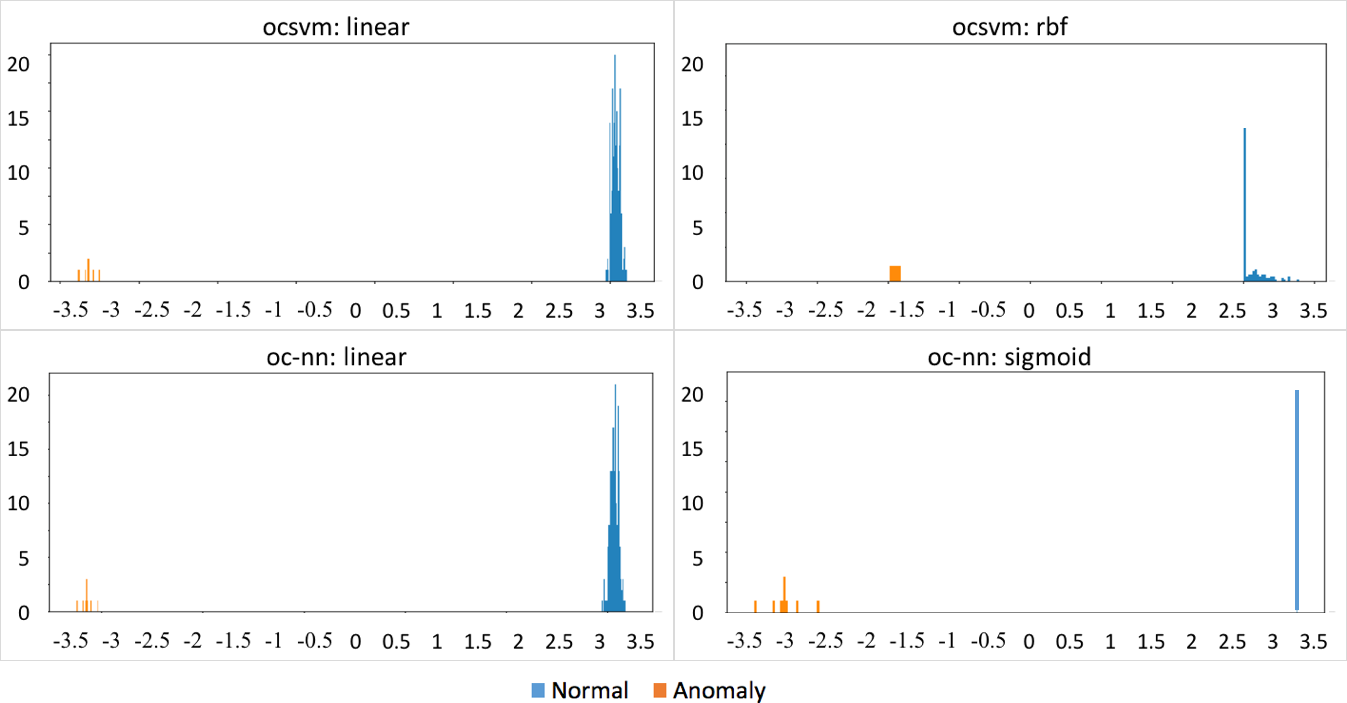
\includegraphics[scale=0.38]{images/s1.png}
    \caption{Decision Score Histogram of anomalous vs normal data points, {\tt synthetic} dataset.}
    \label{fig:synthetic-histogram}
\end{figure}


% Results for Most anomalous and most normal images detected for MNIST dataset
\begin{figure*}
\subfloat[Normal samples detected.  \label{sfig:normalmnistRcae}]{%
  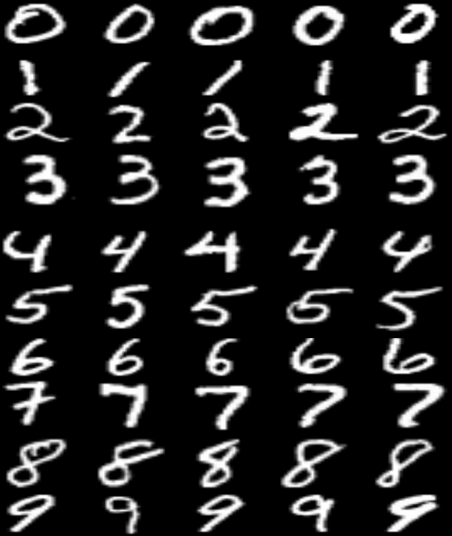
\includegraphics[width=.30\linewidth]{images/mnistNormalRCAE}%
}\hspace{0.5cm}
\subfloat[In-class anomalous samples. \label{sfig:mnistAnomalyRCAE}]{%
  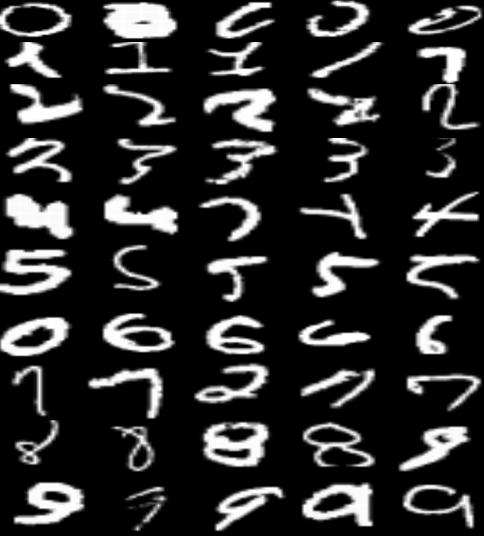
\includegraphics[width=.32\linewidth]{images/mnistAnomalyRCAE}%
}
\caption{MNIST Most normal and in-class anomalous MNIST digits detected by RCAE. }
\label{fig:mnistRCAEresults}
\end{figure*}
%  End of the Figure


% Results for Most anomalous and most normal images detected for MNIST dataset
\begin{figure*}
\subfloat[Normal samples. \label{sfig:mnistnormalOCNN}]{%
  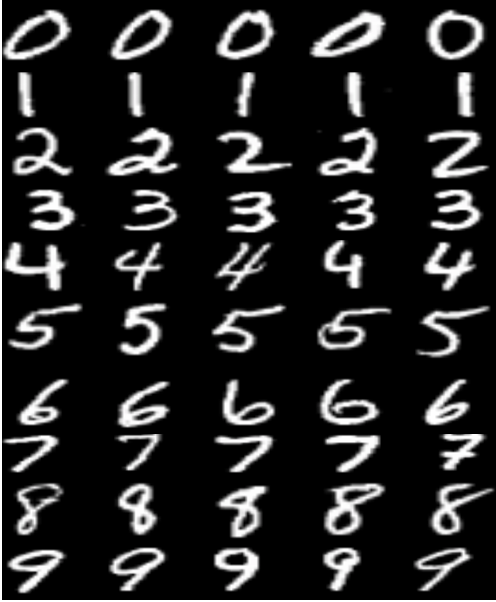
\includegraphics[width=.30\linewidth]{images/mnistnormalOCNN}%
}\hspace{0.5cm}
\subfloat[In-class anomalous samples. \label{sfig:mnistOutlierOCNN}]{%
  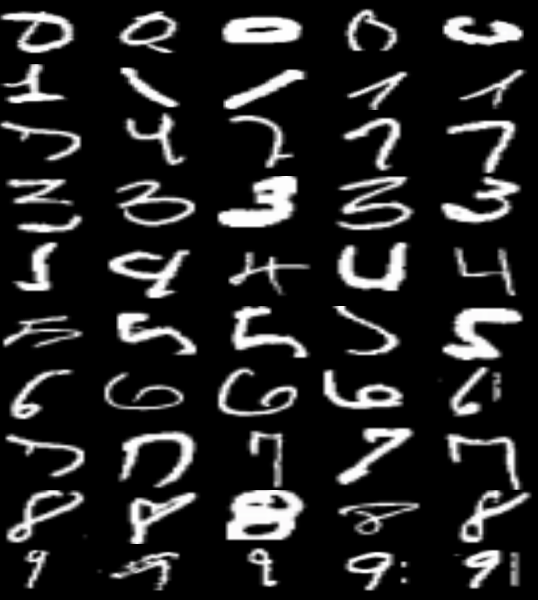
\includegraphics[width=.325\linewidth]{images/mnistOutlierOCNN}%
}
\caption{MNIST Most normal and in-class anomalous MNIST digits detected by OC-NN.}
\label{fig:mnistOCNNresults}
\end{figure*}
%  End of the Figure


%%%%% Mnist Dataset
\subsection{\tt OC-NN on MNIST and CIFAR-10}
\textbf{Setup}
Both MNIST and CIFAR-10  have ten different classes from which we construct one-class classification dataset.  One of the classes is the normal class and
samples from the remaining classes represent anomalies. We use the original training and test splits in our
experiments and only train with training set examples from
the respective normal class. This produces normal instances set of sizes
of n $\approx$ 6000 for MNIST and n $\approx$ 5000 for CIFAR-10 respectively.
Both MNIST and CIFAR-10 test sets have $10000$ samples per class.
The training set comprises of normal instances for each class along with anomalies sampled from
all the other nine classes. The number of anomalies used within training set consists of 1\% normal class for MNIST and  10\% of normal class for CIFAR-10 dataset respectively. We pre-process all images with global contrast normalization using the $L1$
norm and finally rescale to [0, 1] via min-max-scaling.\\
\textbf{Network architectures} For both MNIST and CIFAR-10 datasets, we employ LeNet type
CNNs, wherein each convolutional module consists of a convolutional layer followed by leaky ReLU activations and $2 \times 2$ max-pooling. On MNIST, we use a CNN with two modules, $8\times(5\times5\times1)$-filters followed by $4\times(5\times5\times1)$-filters, and a final dense layer of 32 units. On CIFAR-10,
we use a CNN with three modules, $32 \times (5 \times 5 \times3)$-filters,
$64\times(5\times5\times3)$-filters, and $128\times(5\times5\times3)$-filters, followed
by a final dense layer of $128$ units. We use a batch size of
$200$ and set the weight decay hyperparameter to $ \lambda= 10^{ - 5}$.\\
{\textbf{Results:}}
Results are presented in Table ~\ref{tab:ocnn_results}. RCAE
clearly outperforms both its shallow and deep competitors
on MNIST. On CIFAR-10 the results are convincing but for certain classes the shallow baseline methods outperform the deep models. OC-NN, Soft and One-class Deep SVDD however, shows an overall robust performance. On CIFAR-10 classes such as $AUTOMOBILE$, $BIRD$ and $DEER$ which have less global contrast, as illustrated in Table~\ref{tab:ocnn_results} (indicated in blue color)  OC-NN seems to outperform the shallow methods, Soft and One-class Deep SVDD methods, this is indicative of their future potential on similar data instances.  It is interesting to note that shallow OCSVM/SVDD and KDE perform better than deep methods on two of the ten CIFAR-10 classes. We can see that normal examples of the classes  such as $FROG$ and $TRUCK$ on which OCSVM/SVDD performs best as illustrated in Figure~\ref{fig:ocsvmresults} seem to have strong global structures. For example, TRUCK images are mostly divided horizontally into street and sky, and  $FROG$ have similar colors globally. For these classes,  the performance significantly depends on choice of network architecture. Notably, the One-Class Deep SVDD performs slightly better than its soft-boundary counterpart on both datasets. Figure ~\ref{fig:mnistRCAEresults}, Figure ~\ref{fig:mnistOCNNresults} and Figure ~\ref{fig:cifar10_rcae_results} , Figure ~\ref{fig:cifar10_ocnn_results} show examples of the most normal and most anomalous in-class samples detected by RCAE and OC-NN for MNIST and CIFAR-10 dataset respectively.

% Results for Most anomalous and most normal images detected for CIFAR10 dataset
\begin{figure*}
\subfloat[Normal samples.  \label{sfig:cifar10NormalRCAE}]{%
  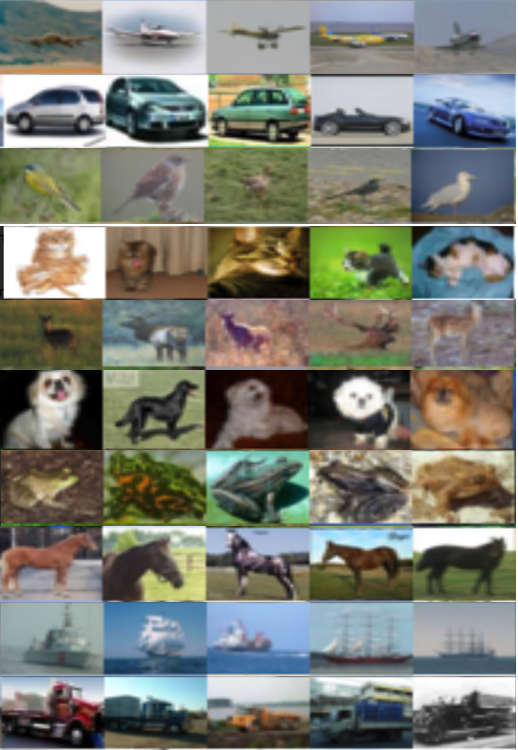
\includegraphics[width=.29\linewidth]{images/cifar10NormalRCAE}%
}\hspace{0.5cm}
\subfloat[In-class anomalous samples. \label{sfig:cifar10AnomalyRCAE}]{%
  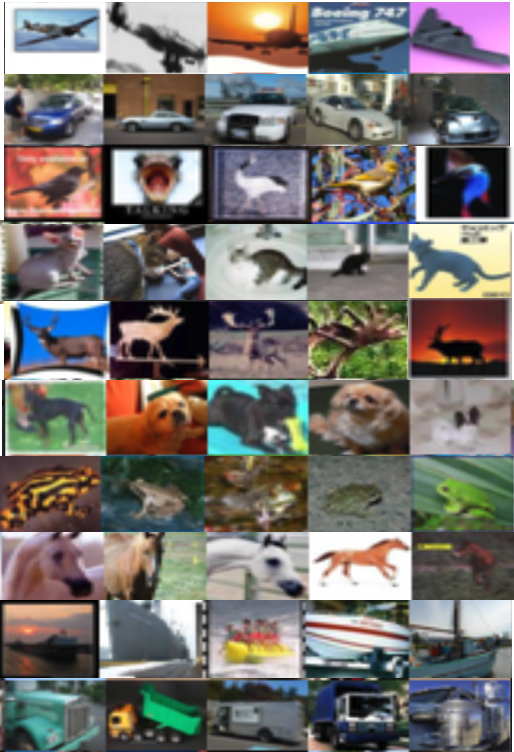
\includegraphics[width=.29\linewidth]{images/cifar10AnomalyRCAE}%
}
\caption{CIFAR-10 Most normal and in-class anomalous CIFAR10 digits detected by RCAE. }
\label{fig:cifar10_rcae_results}
\end{figure*}
%  End of the Figure


% Results for Most anomalous and most normal images detected for CIFAR10 dataset
\begin{figure*}
\subfloat[Normal samples . \label{sfig:cifar10normalOCNN}]{%
  \includegraphics[width=.29\linewidth]{images/cifar10normalOCNN}%
}\hspace{0.5cm}
\subfloat[In-class anomalous samples. \label{sfig:cifar10OutlierOCNN}]{%
  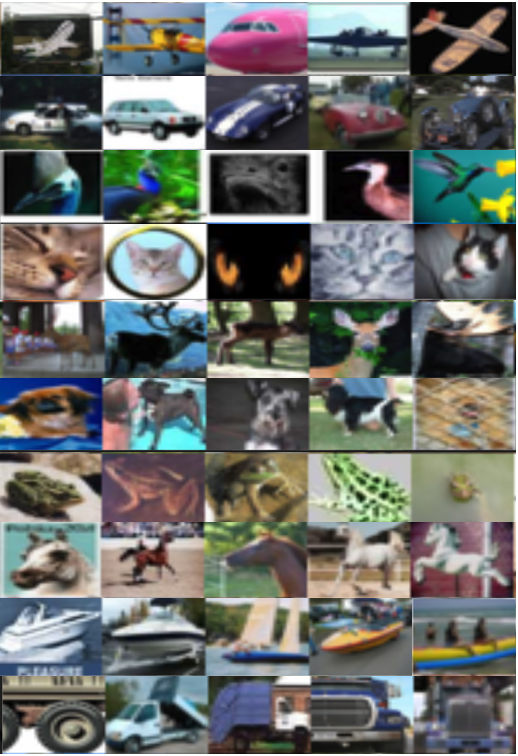
\includegraphics[width=.29\linewidth]{images/cifar10OutlierOCNN}%
}
\caption{CIFAR-10 Most normal and in-class anomalous CIFAR10 digits detected by OC-NN.}
\label{fig:cifar10_ocnn_results}
\end{figure*}
%  End of the Figure

% Results for Most anomalous and most normal images detected for CIFAR10 dataset for
\begin{figure*}
\subfloat[Normal samples . \label{sfig:cifar10normalOCSVM}]{%
  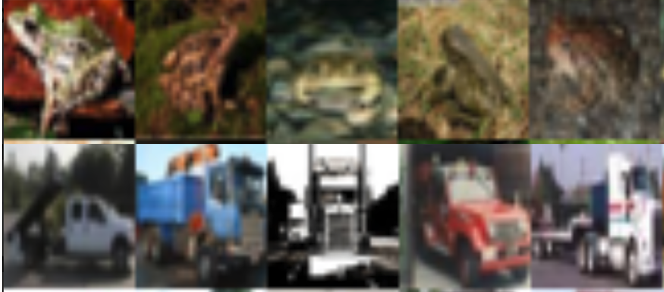
\includegraphics[width=.31\linewidth]{images/cifar10normalOCSVM}%
}\hspace{0.5cm}
\subfloat[In-class anomalous samples. \label{sfig:cifar10OutlierOCSVM}]{%
  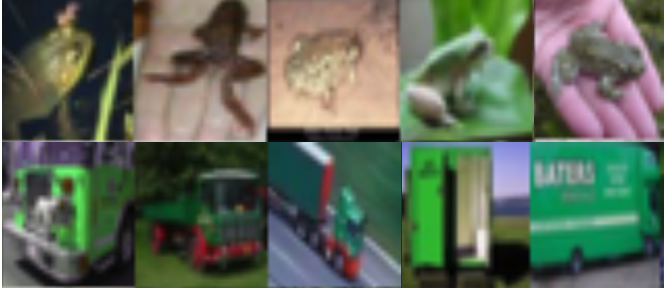
\includegraphics[width=.31\linewidth]{images/cifar10OutlierOCSVM}%
}
\caption{Most normal (left) and most anomalous (right) in-class
examples determined by OCSVM-SVDD for in which OCSVM-SVDD performs best.}
\label{fig:ocsvmresults}
\end{figure*}
%  End of the Figure




\subsection{\tt  Detecting Adversarial attacks on GTSRB stop signs using OC-NN }
\textbf{Setup:}
In many applications (eg. autonomous driving) it is of paramount interest to effectively detect the adversarial samples to ensure safety and security. In this experiment, we
examine  the performance of proposed algorithms on  detecting
adversarial examples. We consider the “stop sign”
class of the German Traffic Sign Recognition Benchmark
(GTSRB) dataset, for which we generate adversarial examples
from randomly drawn stop sign images of the test set
using Boundary Attack~\cite{brendel2017decision}. We create training dataset consists of n = 1150 examples obtained by combining the normal and anomalous samples in both train and test samples. The  number of normal instances n = 1050 stop signs ( 780  from train set +  270 test set ) alongwith  100
adversarial examples are added to obtain training set. We pre-process the
data by removing the 10\% border around each sign, and then resize every image to $32 \times 32$ pixels following the same setup as in ~\cite{pmlrv80ruff18a}. Furthermore, we  apply global contrast normalization using the $L1-norm$ and rescale to the unit interval $[0, 1]$.\\
\textbf{Network architecture} We use a CNN with LeNet architecture having three convolutional modules, $16\times(5\times5\times3)$-filters, $32 \times (5 \times 5 \times 3)$-filters, and $64 \times (5 \times 5 \times 3)$-filters, followed by a final dense layer of 32 units. We train with a smaller batch size of 64, due to the dataset size and set again hyperparamter $\lambda = 10^{ - 6}$.\\
\textbf{Results:}
Results Table ~\ref{tab:gtsrbresults} illustrates the AUC scores obtained. The RCAE outperforms all the other deep models. Figure ~\ref{fig:gtsrbrcaeresults} and Figure ~\ref{fig:gtsrbocnnresults}  shows the most anomalous samples detected by RCAE and OCNN methods respectively, the outliers in this experiment are the images in odd perspectives and the ones that are cropped incorrectly.

\begin{table*}[!t]
   \caption{Average AUCs in \% with StdDevs (over 10 seeds) per method on MNIST and CIFAR-10 dataset.}
   \label{tab:ocnn_results}
   \small % text size of table content
   \centering % center the table
   \begin{tabular}{lccccccccr} % alignment of each column data
   \toprule[\heavyrulewidth]\toprule[\heavyrulewidth]
   \textsc{\pbox{20cm}{Normal \\ Class}} & \textsc{\pbox{20cm}{OCSVM / \\ SVDD}} & \textsc{KDE} &  \textsc{IF} & \textsc{DCAE} & \textsc{ANOGAN} & \textsc{\pbox{20cm}{SOFT-BOUND \\ DEEP SVDD}} & \textsc{\pbox{20cm}{ONE-CLASS \\ DEEP SVDD}} & \textsc{OC-NN} & \textsc{RCAE} \\
   \midrule
   0 & 96.75±0.5 & 97.1±0.0 & 95.32±1.2  & 99.90±0.0 & 96.6±1.3 & 98.66±1.3     & 97.78±0.0 & 97.60±1.7 &
   \bf{99.92±0.0}\\
   1 & 99.15±0.4 & 98.9±0.0 & 99.35±0.0  & 99.96±2.1 & 99.2±0.6 & 99.15±0.0     & 99.08±0.0 & \color[rgb]{0,0,1}99.53±0.0 & \bf{99.97±2.2}\\
   2 & 79.34±2.2 & 79.0±0.0 & 73.15±4.5  & 96.64±1.3 & 85.0±2.9 & 88.09±2.2     & 88.74±1.2 & 87.32±2.1 & \bf{98.01±1.2}\\
   3 & 85.88±1.3 & 86.2±0.0 & 81.34±2.8 & 98.42±0.0 &  88.7±2.1 &  88.93±3.4     & 88.26±3.2 & 86.52±3.9 & \bf{99.25±0.0}\\
   4 & 94.18±1.5 & 87.9±0.0 & 87.40±2.6  & 98.72±0.0 & 89.4±1.3 & 93.88±2.3     & 95.24±1.4 & 93.25±2.4 & \bf{99.23±0.0}\\
   5 & 72.77±3.7 & 73.8±0.0 & 73.96±2.9  & 97.80±1.3 & 88.3±2.9 & 84.35±3.1     & 83.76±3.1 & \color[rgb]{0,0,1}86.48±3.3 & \bf{99.21±0.0}\\
   6 & 95.14±1.1 & 87.6±0.0 & 88.65±0.0  & 99.74±0.0 & 94.7±2.7 & 97.74±0.0     & 97.99±0.0 & 97.12±1.4 & \bf{99.81±1.1}\\
   7 & 91.86±1.6 & 91.4±0.0 & 91.44±1.8  & 99.08±2.2 & 93.5±1.8 & 92.60±1.2     & 93.55±2.3 & 93.64±2.1 & \bf{99.18±0.0}\\
   8 & 88.65±1.2 & 79.2±0.0 & 75.10±3.7  & 96.98±0.0 & 84.9±2.1 & 90.69±3.3     & 90.25±3.1 & 88.54±4.7 & \bf{98.50±2.2}\\
   9 & 92.53±1.9 & 88.2±0.0 & 87.59±1.5  & 98.04±1.3 & 92.4±1.1 & 94.28±2.5     & 94.12±2.4 & 93.54±3.3 & \bf{98.98±1.3}\\
   \hline
  \textsc{Aeroplane}    & 60.37±1.3 & 61.2±0.0 & 63.99±1.1  &71.21±1.5& 67.1±2.5 & 66.15±1.1 & 67.33±2.2 & 60.42±1.9  & \bf{72.04±2.5}\\
   \textsc{Automobile}  & 63.03±1.4 & 63.0±0.0 & 60.56±1.0  &63.05±2.3& 54.7±3.4 & 57.64±3.2 & 58.14±3.1 & \color[rgb]{0,0,1}61.97±2.0  & \bf{63.08±2.1}\\
   \textsc{Bird}        & 63.47±1.0 & 50.1±0.0 & 64.51±1.1  &71.50±1.1& 52.9±3.0 & 61.99±1.4 & 61.35±1.5 & \color[rgb]{0,0,1} {63.66±1.4} & \bf{71.67±1.3}\\
   \textsc{Cat}         & 60.25±0.9 & 56.4±0.0 & 56.16±2.6  &60.57±0.0& 54.5±1.9 & 57.56±4.1 & 55.72±1.4 & 53.57±2.1  & \bf{60.63±1.1}\\
  \textsc{Deer}         & 69.15±0.8 & 66.2±0.0 & 72.66±1.1  &70.85±2.2& 65.1±3.2 & 63.36±1.3 & 63.32±1.2 & \color[rgb]{0,0,1}67.40±1.7  & \bf{72.75±3.3}\\
   \textsc{Dog}         & 66.24±1.5 & 62.4±0.0 & 61.46±2.7  &62.74±2.1& 60.3±2.6 & 58.58±1.2 & 58.68±1.4 & 56.11±2.1  & \bf{63.96±3.3}\\
   \textsc{Frog}        & \bf{71.57±1.5} & {71.3±0.0} & 68.06±2.1  &65.17±4.1& 58.5±1.4 & 63.93±3.1 & 64.45±2.1 & 63.31±3.0  & {64.88±4.2}\\
   \textsc{Horse}       & 63.38±0.8 & 62.6±0.0 & 63.04±1.5  &61.11±1.4& 62.5±0.8 & 60.20±2.2 & 59.80±2.6 & 60.09±2.7  &
   \bf{63.64±0.0}\\
  \textsc{Ship}         & 60.44±1.1 & {65.1±0.0} & 68.01±1.3  &74.18±1.2& 74.68±4.1 & 70.21±1.1 & 67.44±2.2 & 64.67±1.6  & \bf{74.72±1.1}\\
  \textsc{Truck}        & \bf{75.81±0.8} & {74.0±0.0} & 72.83±1.1  &71.36±4.3& 66.5±2.8 & 72.91±3.3 & 68.03±3.2 & 60.32±4.9  & {74.47±1.5}\\
   \bottomrule[\heavyrulewidth]
   \end{tabular}
\end{table*}


% begin of table
\begin{table}[ht]
\caption{Average AUCs in \% with StdDevs (over 10 seeds) per
method on GTSRB stop signs with adversarial attacks.} % title of Table
\centering % used for centering table
\begin{tabular}{l l } % centered columns (4 columns)
\hline\hline %inserts double horizontal lines
\bf{\textsc{Method}} & \bf{\textsc{AUC}}\\ [0.5ex] % inserts table
%heading
\hline % inserts single horizontal line
OC-SVM/SVDD & 52.5 ± 1.3 \\ % inserting body of the table
KDE & 51.5 ± 1.6 \\
IF & 53.37±2.9 \\
AnoGAN & - \\
DCAE & 79.1±3.0 \\
SOFT-BOUND. DEEP SVDD & 67.53±4.7 \\
ONE-CLASS. DEEP SVDD & 67.08±4.7 \\
OC-NN & 63.53±2.5 \\
\bf{\bf{RCAE $\lambda =0$}} &\bf{87.45±3.1} \\
\bf{RCAE} & {$\bf{87.39 \pm 2.7}$} \\ [1ex] % [1ex] adds vertical space
\hline %inserts single line
\end{tabular}
\label{tab:gtsrbresults}
\end{table}
% end of table



% Results for Most anomalous and most normal images detected for GTSRB dataset
\begin{figure*}
\subfloat[Top 50 normal samples.  \label{sfig:normalGtsrb}]{%
  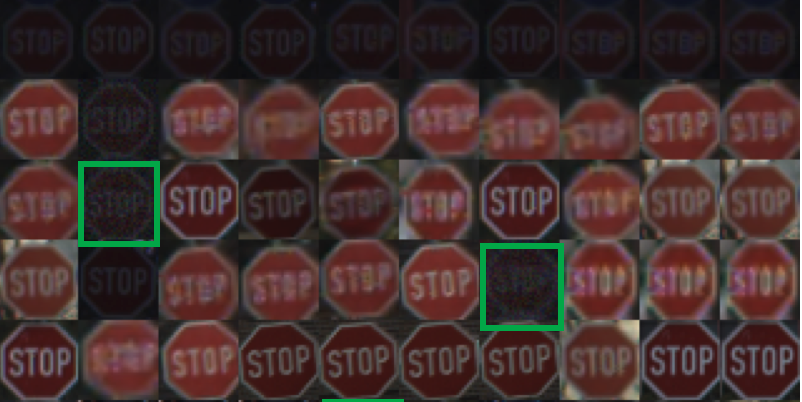
\includegraphics[width=.40\linewidth]{images/most_normalGtsrb}%
}\hspace{0.5cm}
\subfloat[Top 50 anomalous samples. \label{sfig:anomalousGtsrb}]{%
  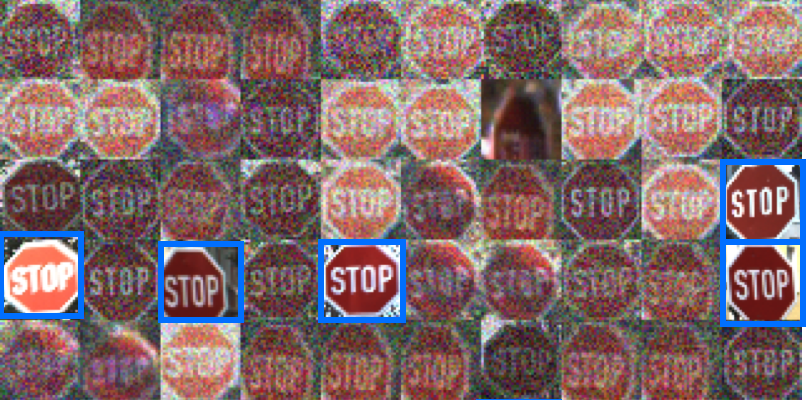
\includegraphics[width=.40\linewidth]{images/most_anomalousGtsrb}%
}
\caption{Most normal and anomalous stop signs detected by RCAE. Adversarial examples are highlighted in green, Normal samples are highlighted in blue}
\label{fig:gtsrbrcaeresults}
\end{figure*}
%  End of the Figure


% Results for Most anomalous and most normal images detected for GTSRB dataset
\begin{figure*}
\subfloat[Top 50 normal samples.. \label{sfig:normalGtsrb}]{%
  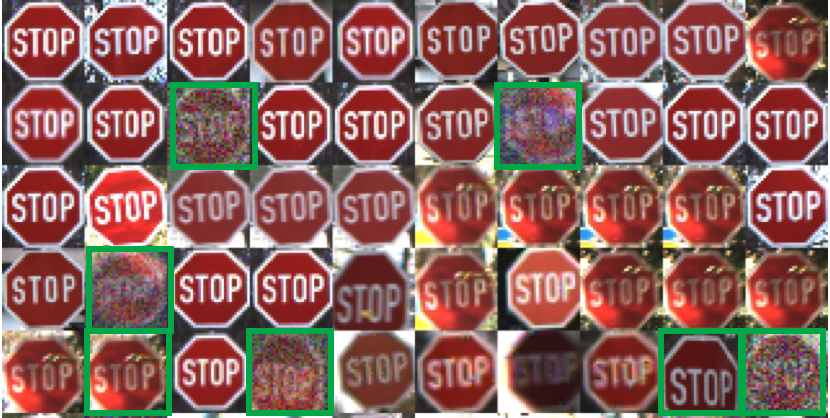
\includegraphics[width=.40\linewidth]{images/most_normalGtsrbocnn}%
}\hspace{0.5cm}
\subfloat[Top 50 anomalous samples. \label{sfig:anomalousGtsrb}]{%
  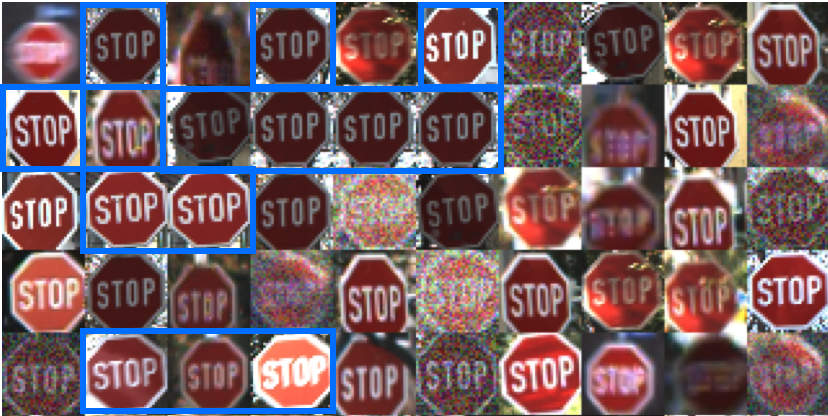
\includegraphics[width=.40\linewidth]{images/most_anomalousGtsrbocnn}%
}
\caption{Most normal and anomalous stop signs detected by OC-NN.  Adversarial examples are highlighted in green, Normal samples are highlighted in blue}
\label{fig:gtsrbocnnresults}
\end{figure*}
%  End of the Figure
